\documentclass[tikz, border=10pt]{standalone}
\usepackage{amsmath}
\usepackage{amsfonts}
\usepackage{amssymb}

\begin{document}

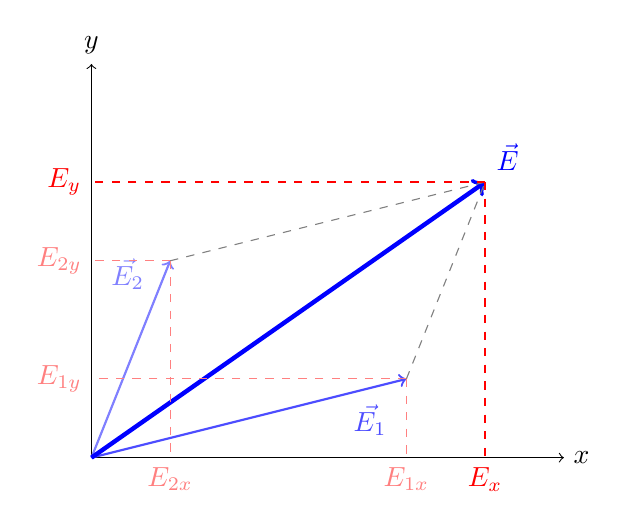
\begin{tikzpicture}
    % Teken het assenstelsel (alleen het eerste kwadrant)
    \draw[->] (0,0) -- (6,0) node[right] {$x$}; % x-as
    \draw[->] (0,0) -- (0,5) node[above] {$y$}; % y-as

    % Definieer de vectoren
    \coordinate (E1) at (4,1);   % Coördinaten van de verlengde vector E1
    \coordinate (E2) at (1,2.5); % Verkorte coördinaten van vector E2
    \coordinate (E) at (5,3.5);  % Nieuwe som van de vectoren E1 + E2

    % Teken de vectoren E1 en E2 in verschillende blauwtinten
    \draw[->, thick, blue!70] (0,0) -- (E1) node[pos=0.8, below right] {$\vec{E_1}$};
    \draw[->, thick, blue!50] (0,0) -- (E2) node[pos=0.8, above left] {$\vec{E_2}$};

    % Teken de som van de vectoren (parallellogramregel) in een andere tint blauw
    \draw[->, ultra thick, blue] (0,0) -- (E) node[pos=1.0, above right] {$\vec{E}$};

    % Teken de parallellogram
    \draw[dashed, gray] (E1) -- (E);
    \draw[dashed, gray] (E2) -- (E);

    % Teken de componenten van E1 in het rood
    \draw[dashed, red!50] (E1) -- (4,0) node[below] {$E_{1x}$}; % x-component van E1
    \draw[dashed, red!50] (E1) -- (0,1) node[left] {$E_{1y}$};  % y-component van E1

    % Teken de componenten van E2 in het rood
    \draw[dashed, red!50] (E2) -- (1,0) node[below] {$E_{2x}$}; % x-component van E2
    \draw[dashed, red!50] (E2) -- (0,2.5) node[left] {$E_{2y}$};  % y-component van E2

    % Teken de componenten van E (de som van de vectoren) in het rood
    \draw[dashed, thick, red] (E) -- (5,0) node[below] {$E_{x}$}; % x-component van E
    \draw[dashed, thick, red] (E) -- (0,3.5) node[left] {$E_{y}$};  % y-component van E

\end{tikzpicture}

\end{document}
